\documentclass{article}
\usepackage[a4paper, margin=2cm]{geometry}

\usepackage{amsmath}
\usepackage{amssymb}
\usepackage{mathtools}
\usepackage{amstext}
\usepackage{amsthm}
\usepackage{fancyhdr}
\usepackage{siunitx}
\usepackage{physics}

\usepackage{hyperref}


\usepackage{graphicx}
\usepackage{float}
\graphicspath{{figures/}} %Setting the graphicspath
\usepackage{float}
\usepackage{caption}
\usepackage{subcaption}

% To work with inkfigures
\usepackage{import}
\usepackage{pdfpages}
\usepackage{transparent}
\usepackage{xcolor}

\newcommand{\incfig}[2][1]{%
    \def\svgwidth{#1\columnwidth}
    \import{./figures/}{#2.pdf_tex}
}

\pdfsuppresswarningpagegroup=1

%\graphicspath{{figures/}}

\pagestyle{fancy}
\rhead{Alexandre Adam}
\lhead{PHY6669 -- Cosmologie \\ Alan Robinson}
\chead{Devoir 3}
\rfoot{\today}
\cfoot{\thepage}

\newcommand{\angstrom}{\textup{\AA}}
\numberwithin{equation}{section}
\renewcommand\thesubsection{\alph{subsection})}
\renewcommand\thesubsubsection{\Roman{subsubsection}}
\newcommand{\s}{\hspace{0.1cm}}

\newcommand{\pyoutput}[2]{#2}

% Astronomy
\DeclareSIUnit\parsec{pc}
\DeclareSIUnit\lightyear{ly}

\begin{document}
\section{Nucléosynthèse}
\subsection{Dodelson ch. 3, Exercice 2}
La densité numérique des électrons-positrons est donnée en terme de la distribution 
de Fermi-Dirac (on conserve les constantes physiques $c,\, \hbar,\, k_B$ pour ce 
sous-numéro):
\begin{equation}\label{eq:nelectron} 
        n_{e^\pm}^{(0)} = g_{e^\pm}\int \frac{d^3p}{(2 \pi \hbar)^{3}} 
        \frac{1}{\exp \left\{ \dfrac{E(p)}{k_B T} \right\} + 1}
\end{equation} 
où $E(p) = \sqrt{p^2 c^2 + m_e^2c^4}$ et $g_{e^\pm} = 2$ pour les états de spins. 
On a négligé le potentiel chimique des électrons $\mu_e$ car il est 
identiquement nul avant et durant la nucléosynthèse.
%dû à notre supposition que 
%le processus $e^- + e^+ \longleftrightarrow \gamma + \gamma$ est à l'équilibre.
À la 
température où la nucléosynthèse se produit ($k_BT \simeq 1\, \text{MeV}$), on ne 
peut pas simplifier l'énergie en faveur de $p$ ou $m_e$ puisque la masse de l'électron
$m_e \simeq 0.5\, \text{MeV}/c^2$ est similaire à la température. 
\begin{figure}[H]
        \centering
        \begin{subfigure}[t]{0.45\textwidth}
                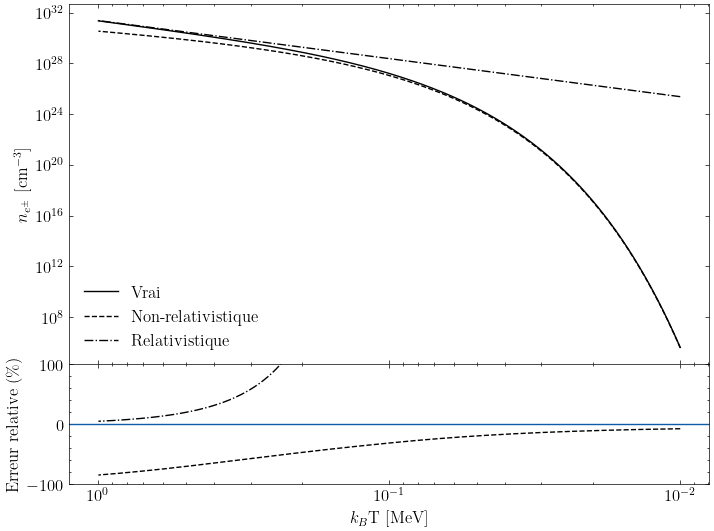
\includegraphics[width=\textwidth]{nucleosynthesis_electron_density}
                \caption{Comparaison des approximations à la vrai fonction durant l'époque de 
                nucléosynthèse.}
                \label{fig:Comparaison}
        \end{subfigure}
        ~
        \begin{subfigure}[t]{0.45\textwidth}
                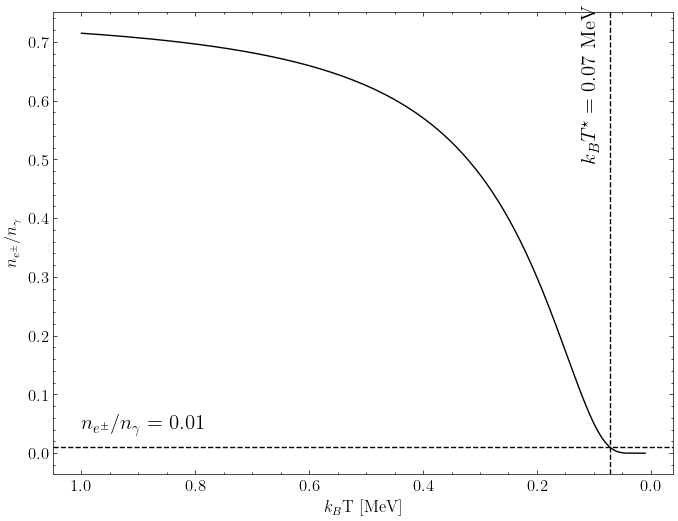
\includegraphics[width=\textwidth]{resultat_ratio_ne_ngamma}
                \caption{Ratio des densités numérique des électrons-positrons 
                lors de l'époque de nucléosynthèse.}
                \label{fig:Res1}
        \end{subfigure}
\end{figure}
La densité numérique des photons se calcule directment à partir de la distribution 
de Planck
\begin{equation}\label{eq:PlanckDensity} 
        n_\gamma^{(0)} = g_\gamma\int_0^{\infty}4\pi\frac{B(\nu, T) d\nu}{h\nu} = 
        \frac{8 \pi }{c^3} g_\gamma \int_0^{\infty } 
        \frac{\nu^2 d\nu}{\exp \left\{ h\nu / k_B T \right\} - 1}
\end{equation} 
Avec substition on retrouve une forme standard pour l'intégrale qui devient
\[
        n_\gamma^{(0)} = g_\gamma\frac{2\zeta(3 )}{\pi^2} \left( \frac{k_B T}{\hbar c} \right)^{3}
\]
où $\zeta(s)$ est la fonction zeta de Riemann.
On cherche la température $T^\star$ à partir de laquelle la densité numérique des électrons 
devient $1\%$ celle des photons $n_\gamma^{(0)}$. En interpolant une grille de valeurs, 
on obtient
\[
        \boxed{k_BT^\star = 0.06\, \text{MeV}}
\]

Avec un ratio de baryons sur photons de
\[
        \eta_b = 6 \times 10^{-10}
\]
au moment de la nucléosynthèse (après annihilation des anti-particules), on peut 
tenter de déterminer le moment (la température) à partir duquel les électrons 
ne seront plus en équilibre avec le processus de création/annihiltion de paires. En 
effet, l'Univers observé est électriquement neutre et on doit avoir $n_{e^{-}} = n_p$ 
à un certains moment. Si on suppose que la grande majorité de la matière baryonique 
est constitué de protons (on néglige les neutrons), alors on trouve
\[
        \boxed{k_B T( \frac{n_{e^{-}}}{n_\gamma} \sim \eta_b) \simeq 0.02\, \text{MeV}}
\]

\subsection{Dodelson ch. 3, Exercice 3}
\subsubsection{Intégrale sur les particules massives}
On cherche à calculer le taux de la conversion de neutrons en protons $\Gamma_{np}$.
Pour ce faire, on estime la section efficace thermal des processus 
$n + \nu_e \longrightarrow p + e^{-}$ et $n + e^{+} \longrightarrow p + \bar{\nu}_e$. 
On néglige la masse de l'électron et on assume que les processus peuvent être 
décrits pas les statistiques de Boltzmann. Dans quel cas leur taux de réaction 
est le même. On considère un seul processus pour le moment et on néglige les 
facteurs de Pauli ($f_i \ll 1$):
\begin{align*}
        \expval{\sigma v} &\equiv \frac{1}{n_n^{(0)} n_{e^{+}}^{(0)}}
        \int \frac{d^{3}\mathbf{p}_n}{(2\pi)^{3}2E_{n}}
        \int \frac{d^{3}\mathbf{p}_{e^{+}}}{(2\pi)^{3}2E_{e^{+}}}
        \int \frac{d^{3}\mathbf{p}_{p}}{(2\pi)^{3}2E_p}
        \int \frac{d^{3}\mathbf{p}_{\bar{\nu}_e}}{(2\pi)^{3}2E_{\bar{\nu}_e}}
        \exp \left\{ - \frac{E_{p_n} + E_{p_{e^{+}}}}{T} \right\}\\
                          &\s\s\s\s\times 
        (2 \pi)^{4} \delta^{(3)}(\mathbf{p}_n + 
        \mathbf{p}_{e^{+}} - \mathbf{p}_p - \mathbf{p}_{\bar{\nu}_e}) 
        \delta(E_{n} + E_{e^{+}} - E_p - E_{\bar{\nu}_e})
        |\mathcal{M}|^{2}
\end{align*}
En négligeant la masse des neutrinos (ce qui est toujours valide) et la masse des 
électrons (valide devant la masse du protons et du neutrons $m_p \sim m_n \sim 2000m_e$), 
alors $E_{e^{+}} = p_{e^{+}} = |\mathbf{p}_{e^{+}}|$ et 
$E_{\bar{\nu}_e} = p_{\bar{\nu}_e}$. De plus,
on approxime l'énergie des particules massive par leur énergie de masse 
$E_p \simeq m_p$ et $E_n \simeq m_n$ ce qui est valide durant la 
nucléosynthèse puisque la température est de $\sim1\, \text{MeV} \ll m_p$.
%Aussi, on peut utiliser la fonction $\delta$ pour remplacer $p_n$ par 
%$p_{\bar{\nu}_e}$ et $p_p$ par $p_{e^{+}}$, ce qui 
%nous laisse
\begin{align*}
        \expval{\sigma v} &= \frac{1}{n_n^{(0)} n_{e^{+}}^{(0)}}
        \int \frac{d^{3}\mathbf{p}_n}{(2\pi)^{3}2m_n}
        \int \frac{d^{3}\mathbf{p}_{e^{+}}}{(2\pi)^{3}2p_{e^{+}}}
        \int \frac{d^{3}\mathbf{p}_{p}}{(2\pi)^{3}2m_p}
        \int \frac{d^{3}\mathbf{p}_{\bar{\nu}_e}}{(2\pi)^{3}2p_{\bar{\nu}_e}}
        \exp \left\{ - \frac{m_n + p_{e^{+}}}{T} \right\}\\
                          &\s\s\s\s\times 
        (2 \pi)^{4 } \delta^{(3)}(\mathbf{p}_n + 
        \mathbf{p}_{e^{+}} - \mathbf{p}_p - \mathbf{p}_{\bar{\nu}_e}) 
        \delta(\mathcal{Q} + p_{e^{+}} - p_{\bar{\nu}_e})
        |\mathcal{M}|^{2}
\end{align*}
où on a définit $\mathcal{Q} = m_n - m_p = 1.293\, \text{MeV}$. On fait l'intégrale 
sur l'espace de phase des particules massives sur une coquille dans 
le système de référence du neutron (le choix est libre puisque 
l'intégrale est un invariant de Lorentz), de sortes que $\mathbf{p}_n = 0$. 
La fonction $\delta $ de Dirac restante sélectionne alors 
$\mathbf{p}_{e^{+}} = \mathbf{p}_p + \mathbf{p}_{\bar{\nu}_e}$ par 
conservation de la quantité de mouvement et on obtient (en appliquant 
la fonction $\delta^{3}$ sur $\int d^{3}\mathbf{p}_p$):

\begin{align*}
        \expval{\sigma v} &= \frac{1}{n_n^{(0)} n_{e^{+}}^{(0)}}
        \frac{2\pi}{ 4m_n m_p}
        \int \frac{d^{3}\mathbf{p}_n}{(2\pi)^{3}}
        \int \frac{d^{3}\mathbf{p}_{e^{+}}}{(2\pi)^{3}2p_{e^{+}}}
        \int \frac{d^{3}\mathbf{p}_{\bar{\nu}_e}}{(2\pi)^{3}2p_{\bar{\nu}_e}}
        \exp \left\{ - \frac{m_n + p_{e^{+}}}{T} \right\}\\
                          &\s\s\s\s\times 
        \delta(\mathcal{Q} + p_{e^{+}} - p_{\bar{\nu}_e})
        |\mathcal{M}|^{2}
\end{align*}
À l'équilibre, 
\[
        n_n^{(0)} = 2\int \frac{d^{3}\mathbf{p}_n}{(2\pi)^{3}}\exp \left\{ -\frac{m_n}{T} \right\}
\]
De sortes que 
\begin{align*}
        \Aboxed{\expval{\sigma v} &= \frac{1}{n_{e^{+}}^{(0)}}
        \frac{\pi}{ 4m_n m_p}
        \int \frac{d^{3}\mathbf{p}_{e^{+}}}{(2\pi)^{3}2p_{e^{+}}}
        \int \frac{d^{3}\mathbf{p}_{\bar{\nu}_e}}{(2\pi)^{3}2p_{\bar{\nu}_e}}
        \exp \left\{ - \frac{p_{e^{+}}}{T} \right\}
        \delta(\mathcal{Q} + p_{e^{+}} - p_{\bar{\nu}_e})
|\mathcal{M}|^{2}}
\end{align*}


\subsubsection{Taux de réaction}
L'amplitude de la réaction est
\begin{equation}\label{eq:AmpReaction} 
        |\mathcal{M}|^{2} = 32 G_F^2(1 + 3g_A^2)m_p^2p_{\nu}p_e
\end{equation} 
où $g_A$ est le vecteur axial de couplage du nucléon qu'on mesure 
aujourd'hui via le temps de vie du neutron
\[
        \tau_n^{-1} = \lambda_0G_F^2(1 + 3g_A^2) \frac{m_e^5}{2\pi^3}
\]
où $\lambda_0 \simeq 1.636$ et $\tau_n = 879.4 \pm 0.6\,\, \text{s}$ et 
$G_F$ est la constante de Fermi
\[
        G_F = 1.16639(1) \times 10^{-5}\, \text{GeV}^{-2} (\hbar c)^{3}
\]
On performe 
l'intégrale de la section efficace thermalisée sur une 
coquille dans l'espace de phase du positron. On applique en 
premier lieu la fonction $\delta $ sur l'énergie:
\begingroup
\allowdisplaybreaks
\begin{align*}
        n_{e^{+}}^{(0)}\expval{\sigma v} &= 
        \frac{32\pi G_F^2(1 + 3g_A^2) m_p}{ 4m_n}
        \int \frac{d^{3}\mathbf{p}_{e^{+}}}{(2\pi)^{3}2p_{e^{+}}}
        \int \frac{d^{3}\mathbf{p}_{\bar{\nu}_e}}{(2\pi)^{3}2p_{\bar{\nu}_e}}
        \exp \left\{ - \frac{p_{e^{+}}}{T} \right\}
        \delta(\mathcal{Q} + p_{e^{+}} - p_{\bar{\nu}_e})
        p_{\bar{\nu}_e} p_{e^{+}} \\
        &= 
        \frac{32\pi G_F^2(1 + 3g_A^2) m_p}{ 4m_n}
        \int_0^{\infty } \frac{4 \pi p^2_{e^{+}} dp_{e^{+}}}{(2\pi)^{3}2p_{e^{+}}}
        \int_0^{\infty } \frac{4 \pi p^2_{\bar{\nu}_e} dp_{\bar{\nu}_e}}{(2\pi)^{3}2p_{\bar{\nu}_e}}
        \exp \left\{ - \frac{p_{e^{+}}}{T} \right\}
        \delta(\mathcal{Q} + p_{e^{+}} - p_{\bar{\nu}_e})
        p_{\bar{\nu}_e} p_{e^{+}} \\
        &= 
        \frac{4 G_F^2(1 + 3g_A^2) m_p}{ (2\pi)^{3}m_n}
        \int_0^{\infty }  p^2_{e^{+}} dp_{e^{+}}
        \int_0^{\infty }  p^2_{\bar{\nu}_e} dp_{\bar{\nu}_e}
        \exp \left\{ - \frac{p_{e^{+}}}{T} \right\}
        \delta(\mathcal{Q} + p_{e^{+}} - p_{\bar{\nu}_e})
        \\
        &= 
        \frac{4 G_F^2(1 + 3g_A^2) m_p}{ (2\pi)^{3}m_n}
        \int_0^{\infty }  dp_{e^{+}} p^2_{e^{+}} 
        (\mathcal{Q} + p_{e^{+}})^2
        \exp \left\{ - \frac{p_{e^{+}}}{T} \right\}
\end{align*}
\endgroup
On applique la substitution $y \equiv \dfrac{p_{e^{+}}}{T}$ pour obtenir
\begin{align*}
        n_{e^{+}}^{(0)}\expval{\sigma v} &= 
        \frac{4 G_F^2(1 + 3g_A^2) m_p}{ (2\pi)^{3}m_n}T^3
        \int_0^{\infty }  dy\,\, y^2  (\mathcal{Q}^2 + 2\mathcal{Q}Ty + T^2y^2)
        e^{-y}
\end{align*}
On reconnaît la forme intégrale de la fonction $\Gamma(s)$, ainsi
\begin{align*}
        n_{e^{+}}^{(0)}\expval{\sigma v} &= 
        \frac{4 G_F^2(1 + 3g_A^2) m_p}{ (2\pi)^{3}m_n}T^3
        \left[ \mathcal{Q}^{2}\Gamma(3) + 2 \mathcal{Q}T \Gamma(4)
        + T^2 \Gamma(5)\right] \\
        &= 
        \frac{4 G_F^2(1 + 3g_A^2) m_p}{ (2\pi)^{3}m_n}T^3
        \left[ 2\mathcal{Q}^{2} + 12 \mathcal{Q}T
        + 24T^2 \right] \\
        &= 
        \frac{16 \pi^3 m_p}{ \lambda_0(2\pi)^{3}\tau_n m_e^5 m_n}T^3
        \left[ \mathcal{Q}^{2} + 6 \mathcal{Q}T
        + 12T^2 \right] \\
\end{align*}
%Avec les valeurs numériques mentionnées plus haut, on trouve le facteur lié au 
%vecteur de couplage axial:
%\[
        %\boxed{ 1 + 3g_A^2 = 23.9}
%\]
En posant de plus $x \equiv \dfrac{\mathcal{Q}}{T}$, on trouve
\[
        \boxed{\Gamma_{np} = 2 n_{e^{+}}^{(0)} \expval{\sigma v} 
        = 
        \frac{ 4 m_p \mathcal{Q}^5}{ \lambda_0 \tau_n m_e^5 m_n} \frac{1}{x^5}
        \left[ x^2 + 6x 
+ 12 \right]}
\]
On peut comparer avec l'équation (3.29) et on remarque qu'on 
obtient
\[
        \boxed{\Gamma_{np} \simeq \frac{253.57}{\tau_n x^5} \left[ x^2 + 6x + 12 \right]}
\]
La constante numérique $253$ est comparable à $255$, 
celle obtenue par Bernstein (1988).
%\citet{Bernstein1988}.




\end{document}

